Operating large-scale clusters is expensive both in terms of
investment to buy all the necessary hardware equipment but also in terms of
human resources that will maintain them. The variety in the jobs
running in a big organization poses a great challenge in the
utilization and efficiency of a cluster. There are long-running
production jobs that should ``never'' stop running, short-living
memory intensive batch jobs that analyze massive amount of data,
testing jobs running with the lowest priority and so forth. At the
same time schedulers should be able to scale to tens of thousands of
nodes per cluster and be highly available with minimum downtime. In order
to tackle these issues there has been a lot of research regarding cluster
schedulers or data center operating systems as they are also
referred. In this section three different architectures will be presented,
based on the taxonomy published
in the Omega paper \cite{41684}. An overview of these architectures is
depicted in Figure \ref{fig:sch_tax}.

\begin{figure}
\centering
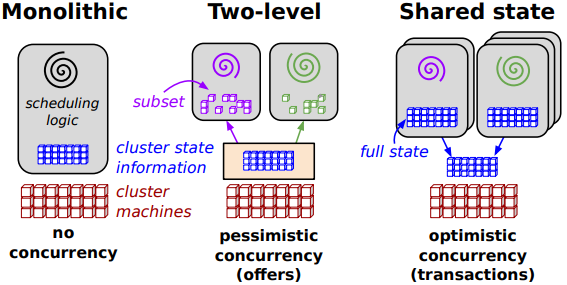
\includegraphics[scale=0.6]{resources/images/Background/schedulers_taxonomy.png}
\caption{Cluster schedulers architecture \cite{41684}}
\label{fig:sch_tax}
\end{figure}

\subsection{Monolithic}
\label{ssec:tax_monolithic}
The first category of schedulers explored is the \emph{monolithic}. In
this architecture there is a single, centralized entity that makes all
the scheduling decisions with no parallelism. A monolithic scheduler
still can facilitate different scheduling policies according to the type
of the workload by providing multiple code paths. Depending on the
type of the job, the execution flow can take different path --
policy. Although, it is tempting to support multiple
scheduling policies, ``it is surprisingly difficult to support a wide
range of policies in a sustainable manner using a single-algorithm
implementation'' \cite{41684}.

Another drawback of monolithic schedulers is the head-of-line
blocking. A small and easy to schedule job might get stack behind a
big and demanding job. This will delay the execution of the former, a
side effect that is not desirable in the enterprise world. Scalability
is another issue that has to be addressed. Since the scheduler runs on
a single instance it can be the bottleneck if the cluster size is big
enough. On the other hand, a monolithic scheduler has a full view of the
cluster and its available resources. For that reason it can make
optimal decisions on the job placement and achieving high utilization
(until it becomes the bottleneck).

A slight variation of a monolithic scheduler is the static
partitioning of the cluster. Each partition will run its own
monolithic scheduler with a separate policy according to the jobs
type. This approach though leads to fragmentation and sub-optimal
cluster utilization.

A prominent example of a monolithic scheduler is Apache Hadoop YARN
and Hops-YARN. The key distinguishing characteristic of Hops-YARN is that the state of the
scheduler is stored in the MySQL Cluster which opens the way for
various architectural experimentations resembling shared state schedulers (see
Section \ref{ssec:tax_shared_state}).

\subsection{Two-level}
\label{ssec:tax_two_level}
The direct shortcoming of the monolithic scheduler is the inability to
keep up with the diverse job types since it can only run one
scheduling policy. The \emph{two-level} scheduling architecture tries
to fix it by dynamically partition the cluster and adjust the
partitions while each partition runs its own \emph{scheduling framework}. This approach
is explored by systems like Mesos \cite{Hindman:2011:MPF:1972457.1972488}
and Hadoop-on-Demand \cite{hadoop_hod}.

The resource allocator dynamically partitions the cluster and offers
the available resources of that particular partition to
the \emph{scheduling framework} running on top of it. That way, at any
time a resource is examined for possible allocation by only one
framework. In essence that means that the framework holds a lock on a
partition's resources for as long as the scheduling decision lasts. This
can be an issue in terms of cluster utilization and scheduling time
with long running tasks or heavy resource requirements. Finally, as
the framework does not have access to the full view of the cluster it
cannot preempt containers belonging to another partitions in favour of
high priority, heavy tasks.

\subsection{Shared state}
\label{ssec:tax_shared_state}
Last but not least in the taxonomy of schedulers is the \emph{shared
state} scheduling with systems such as Omega \cite{41684} and Borg
\cite{43438}. In this category there are multiple schedulers, each
running different scheduling policies, like in two-level scheduling but
the main difference is that every scheduler operates on the full view of
the cluster. Compared to two-level, optimistic concurrency control is
used to deal with state updates increasing the scheduler
parallelism. This comes with the risk of re-scheduling the job in case
of a conflicting state between two or more schedulers.

In Omega they realize it using a persistent storage for the
allocations in the cluster called \emph{cell state}. Each scheduler
has a local, frequently updated copy of it, on which it operates in
order to make its decision. When a scheduler assigns some resources to
a job, it updates the shared state in a transactional way. If during scheduling
another scheduler has assigned those resources, then the
transaction is rolled-back and the request has to be re-scheduled. On a
successful decision, the allocation is persisted in the shared state
and other schedulers will update their local copy asynchronously. The
commit is atomic and at most one transaction will succeed. To
prevent starvation, a scheduler will accept all but the conflicting
resources. It will synchronize its local copy with the shared one and
in a next round it will try to allocate the rest of the requested
resources. That way schedulers work completely independently,
maximizing parallelism. Clearly the performance of this type of
schedulers is determined by the ratio of ultimately failed allocations
over the successful.
